\section{Examples of derivable functions}\label{sec:AppendixExamples}
To illustrate derivable functions, we present a series of examples, some of them will be useful later.

\noindent \begin{example}[Identity] For every type $\rSigma$, the identity function $x\in\rSigma\mapsto x\in\rSigma$ is derivable. This is achieved by induction on the types: the identity function over a finite set of elements is derivable since its domain is finite. %, and the identity function over $\llone$ is the first-order function $!$.
For every types $\rSigma$ and $\rGamma$, the identity
function over $\ranked{\rSigma+\rGamma}$ is the disjoint union of the co-projections $\ranked{\rSigma \to \rSigma + \rGamma}$ and $\ranked{\rGamma \to \rSigma + \rGamma}$. The
identity function over $\ranked{\rSigma \times \rGamma}$ is the pairing of the projections $\ranked{\rSigma \times \rGamma \to \rSigma}$ and $\ranked {\rSigma \times \rGamma \to \rGamma}$. The
identity function over $\ranked{\rSigma \otimes \rGamma}$ is the tensor product of the identity over $\rSigma$ and the identity over $\rGamma$. Finally,
the identity function over $\tmonad\rSigma$ and $\reduce k$ are constructed from the identity function over $\rSigma$ using the combinators $\tmonad$ and $\reduce k$ respectively.
\end{example}


\bigskip
\noindent\begin{example}[Filter]\label{ex:filter} Consider the types $\rGamma, \rSigma$  where $\rGamma$ is a finite type of unary symbols. Consider the function:
$$ \ranked{f:\tmonad (\rSigma+\rGamma)\to\tmonad \rSigma}$$
which erases the elements of $\rGamma$ from the inupt tree. This function is well defined since erasing unary symbols does not break the tree structure of the input. 
Let us explain why this is a derivable function. 
Consider the basic functions $\ranked{\unit_\rSigma:\rSigma\to\tmonad\rSigma}$ and the constant function $\ranked{\mathsf{empty}:\rGamma\to\tmonad\rSigma}$ which associates to every element of $\rGamma$ the tree reduced to the variable $x_1$. Using the cases combinator, we get a tree in $\tmonad\tmonad\rSigma$, which we transform into a tree in $\tmonad \rSigma$ using the flattening function $\flatt_\rSigma$.
\end{example}


\bigskip
\noindent \begin{example}[Pattern matching]\label{ex:patternMatching} 
\end{example}


\bigskip
\noindent \begin{example}[Parent and sibling informations]  Let $\rGamma$ be a finite type. We define $\ranked{\rGamma_0}$  to be the ranked set obtained from $\rGamma$ by setting the arity of every element to $0$.  
\medskip
Consider the function:
$$\ranked{ \mathsf{Parent}: \tmonad \rGamma \to \tmonad (\rGamma\otimes (\rGamma_0+\bot))}$$
which adds to every node of a term in $\tmonad \rSigma$ the label  of its parent if it has one and $\bot$ if it is the root.

% from  $(\rGamma\cup\bot)^{\leq n}$, whose lenght is the arity of the node, and such that the $i^{th}$ element of the  list is the symbol of its $i^{th}$ sibling if it has one, otherwise it is $\bot$.
Let us explain why $\ranked{\mathsf{Parent}}$ is derivable. 
\begin{enumerate}
\item For every symbol $a\in \rGamma$, consider the unary symbols $a_\#$ and $a_\$$.
We set $\ranked{\rGamma_\#}=\{a_\#\mid a\in\rGamma\}$ and $\ranked{\rGamma_\$}=\{a_\$\mid a\in\rGamma\}$.
Let $g$ be the following function:
 \begin{align*}
\ranked{  g: \rGamma} &\ranked{\to \tmonad(\rGamma+\rGamma_\#+\rGamma_\$)}\\
  a &\mapsto a_\#\tensorpair{a\tensorpair{a_\$\tensorpair{x_1},\dots,a_\$\tensorpair{x_{\mathsf{arity(a)}}}}}.
\end{align*}
The action of $\ranked{g}$ on a $\rGamma$ symbol looks like this:
\begin{center}
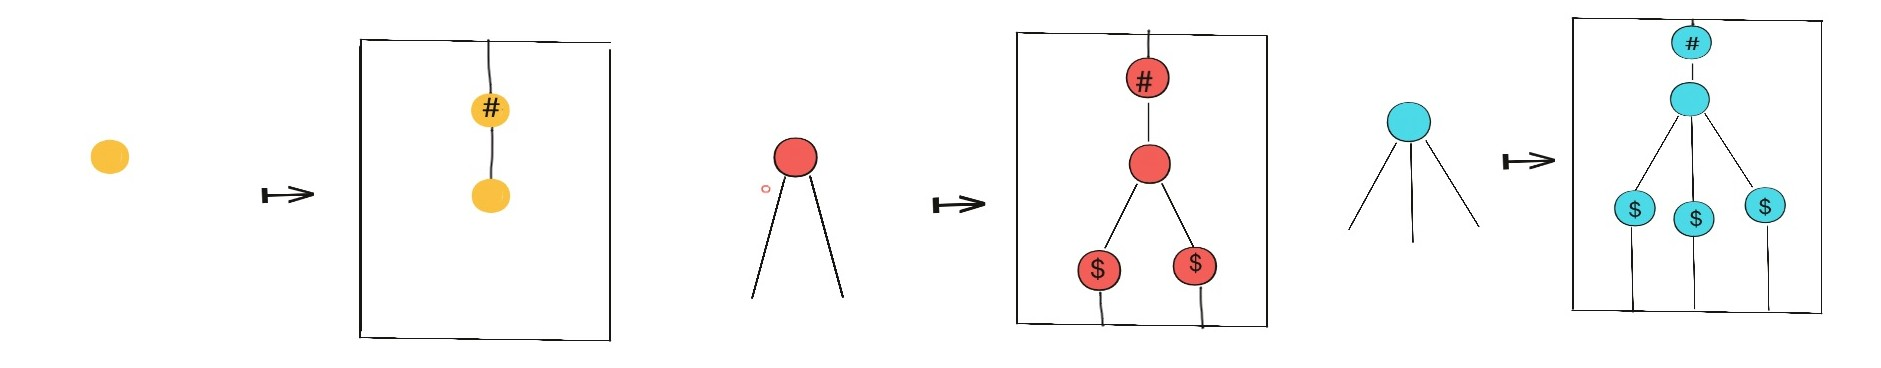
\includegraphics[scale=.15]{MyPic1.jpg}
\end{center}
\item We lift $\ranked{g}$ to the terms of $\tmonad \rGamma$ using the combinator $\tmonad$, then we apply a flattenig. After this operation, a term in $\tmonad\rGamma$ is transformed to a term in $\ranked{\tmonad(\rGamma+\rGamma_\#+\rGamma_\$)}$ this way:
\begin{center}
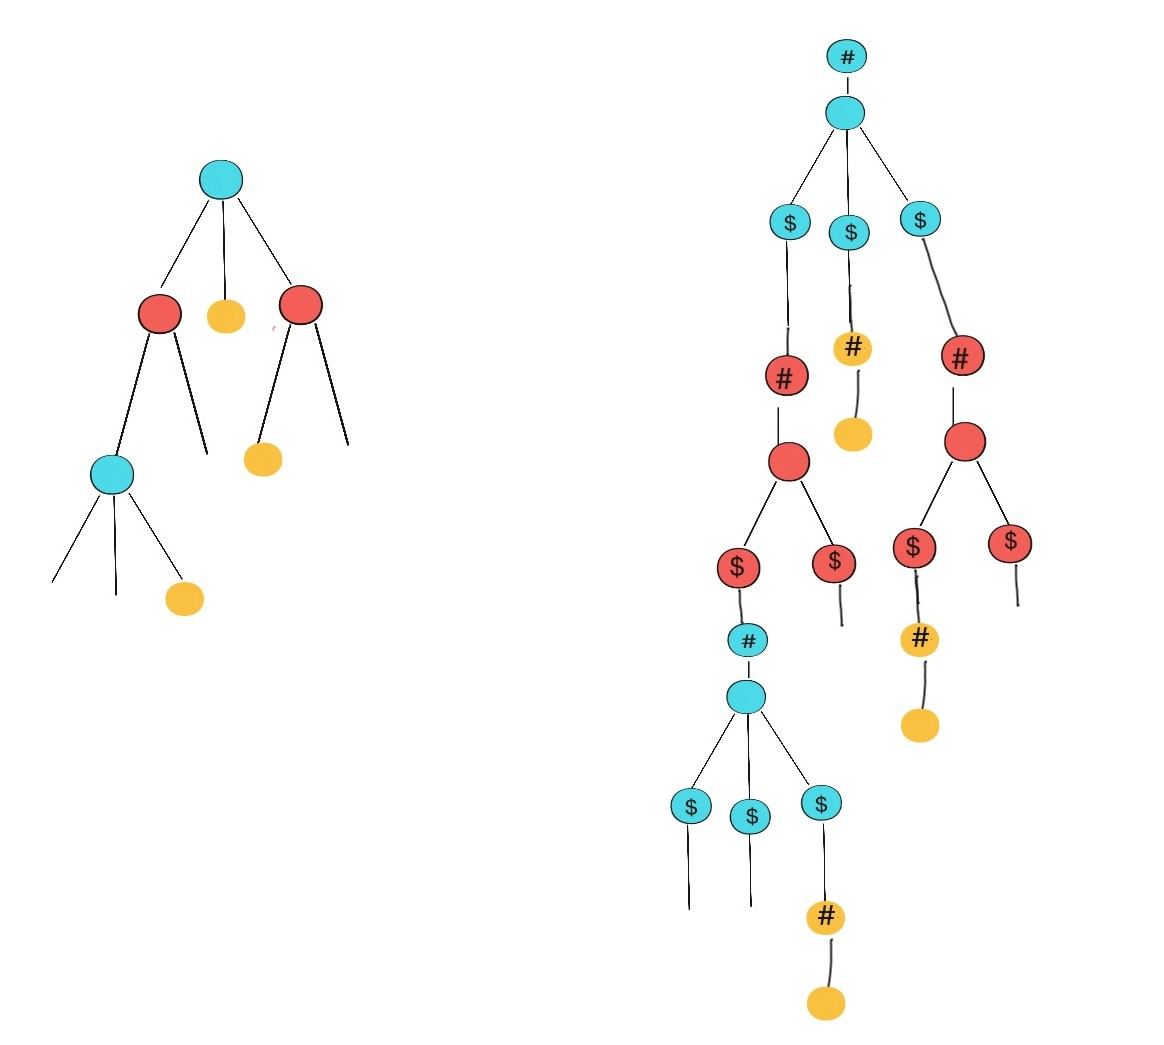
\includegraphics[scale=.15]{MyPic2.jpg}
\end{center}
\item We apply $\ancfact$, to separate the symbols of $\rGamma$ form the symbols of $\ranked{\rGamma_\#}$ and $\ranked{\rGamma_\$}$, we get then a term in $\ranked{\tmonad(\tmonad\rGamma+\tmonad(\rGamma_\#+\rGamma_\$))}$. Those terms look like this:
\begin{center}
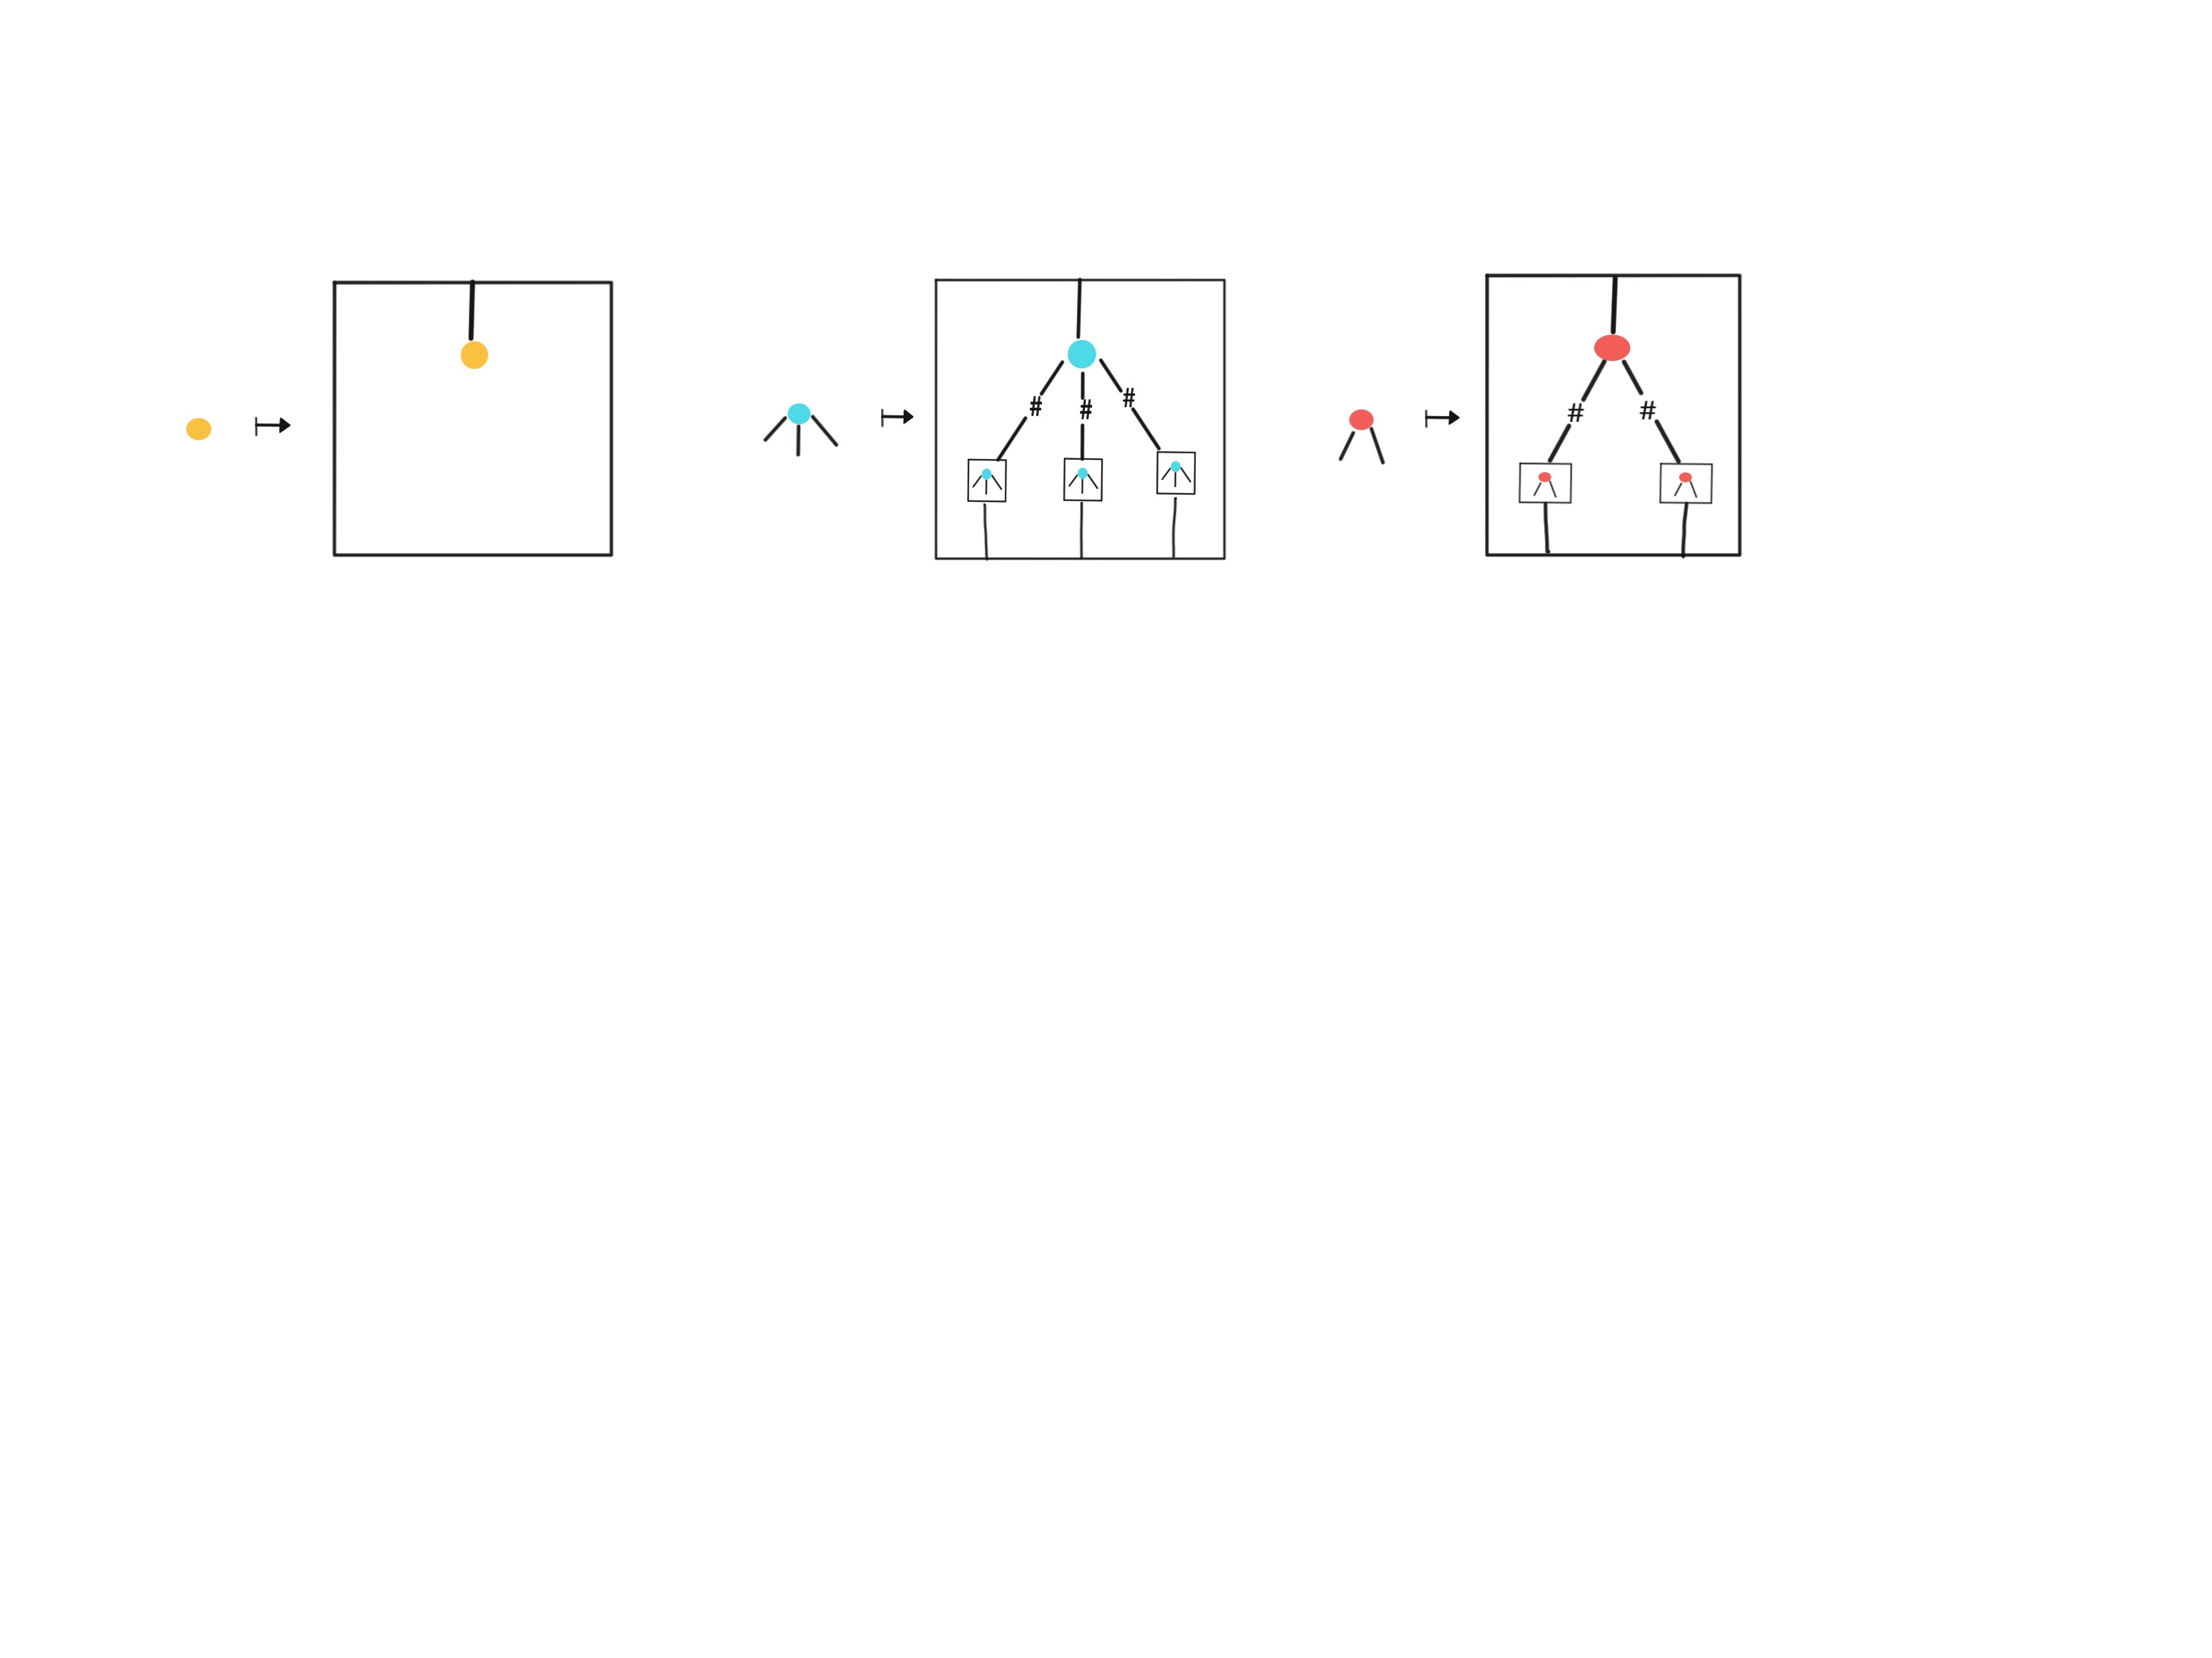
\includegraphics[scale=.15]{MyPic3.jpg}
\end{center}
\item Consider the function $\ranked{h:\tmonad(\rGamma_\#+\rGamma_\$)\to \tmonad(\rGamma_\#+\rGamma_\$)}$ which maps
\begin{align*}
a_\$\tensorpair{b_\#\tensorpair{x_1}} &\mapsto b_\$\tensorpair{a_\$\tensorpair{x_1}}&  a, b\in \rGamma\\
a_\$\tensorpair{x_1} & \mapsto  x_1&  a\in\rGamma
\end{align*}
and leaves the other terms unchanged. 
The function $\ranked{h}$ is derivable thanks to the pattern-matching construction of Example~\ref{ex:patternMatching}.

\item To the factors of type $\tmonad \rGamma$ we apply the identity function, and to the factors $\ranked{\tmonad(\rGamma_\#+\rGamma_\$)}$ we apply $\ranked{h}$. After that, we inject the factors into $\ranked{\tmonad(\rGamma+\rGamma_\#+\rGamma_\$)}$ then we apply a flattening to get terms in $\ranked{\tmonad(\rGamma+\rGamma_\#+\rGamma_\$)}$ having the form:
\begin{center}
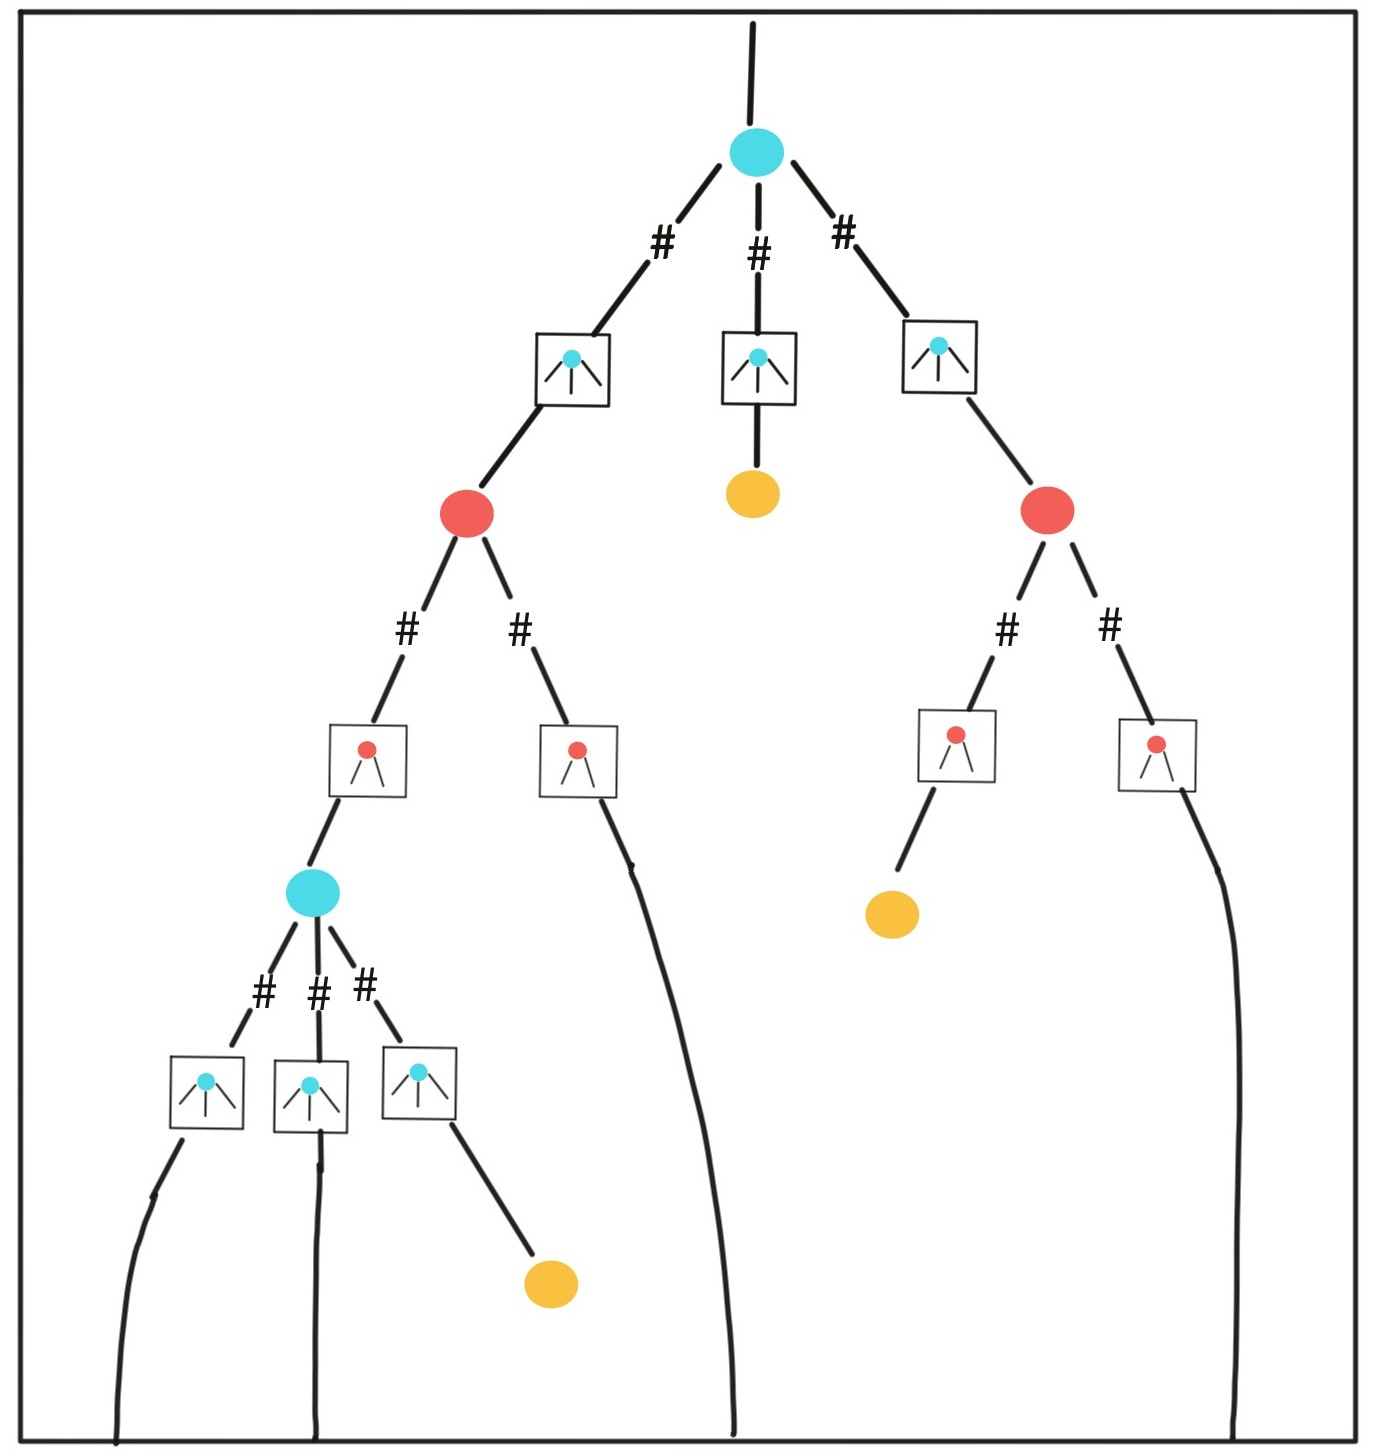
\includegraphics[scale=.15]{MyPic4.jpg}
\end{center} 
\item We apply $\ancfact$ to separate the symbols of $\ranked{\rGamma_\$}$ form the others. Doing so, every $\rGamma$ node ends up in the same factor as its parent (marked with $\$ $):
\begin{center}
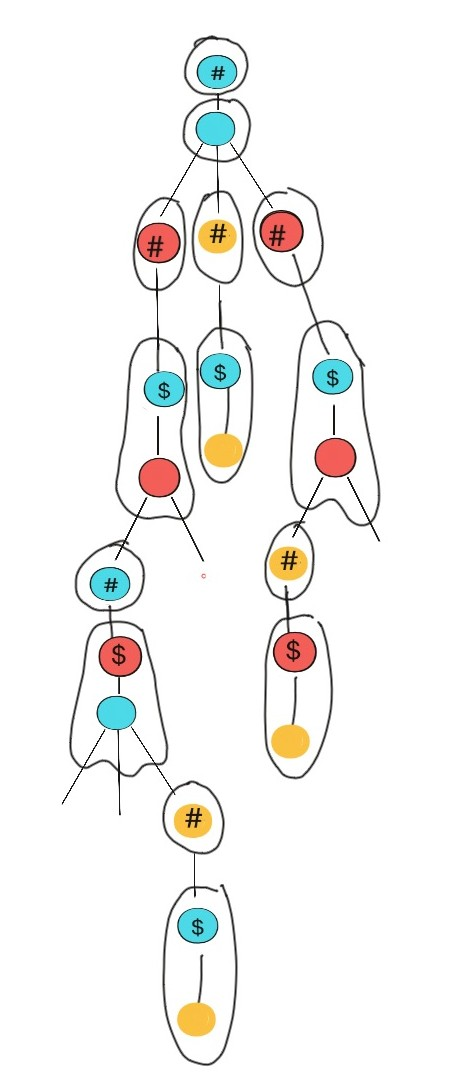
\includegraphics[scale=.15]{MyPic5.jpg}
\end{center}
\item Consider the function $\ranked{k:\tmonad(\rGamma+\rGamma_\#)\to \rGamma\otimes(\rGamma_0+\bot)+\tmonad(\rGamma+\rGamma_\#)}$ which maps
\begin{align*}
a\tensorpair{x_1,\dots,x_n} \mapsto \tensorpair{a,\bot}\tensorpair{x_1,\dots,x_n} \\
b_\$\tensorpair{a\tensorpair{x_1,\dots,x_n}} \mapsto \tensorpair{a,b}\tensorpair{x_1,\dots,x_n} 
\end{align*}
and leaves the terms other unchanged. We apply the function $\ranked{k}$ to the $\ranked{\tmonad(\rGamma+\rGamma_\#)}$
factors and the identity to the others. After several applications of injections and flattening, we get a term in $\ranked{\tmonad(\rGamma\otimes(\rGamma_0+\bot)+\rGamma_\#+\rGamma_\$+\rGamma)}$. We erase the symbols of $\ranked{\rGamma_\$}$ and $\ranked{\rGamma_\#}$  using the filter function from Example~\ref{ex:filter}, and obtain a term in $\ranked{\tmonad(\rGamma\otimes(\rGamma_0+\bot)+\rGamma)}$. 
We get rid of the symbols of $\rGamma$ in the output type, we apply any derivable function of type $\ranked{\rGamma\to \rGamma\otimes(\rGamma_0+\bot)}$, for example the one defined by:
\begin{align*}
a \mapsto \tensorpair{a,\bot}
\end{align*}
 Doing so we get the desired function.
\end{enumerate}
\medskip

Now consider the function $$Par:\tmonad\rGamma\to \tmonad (\rGamma\otimes \rGamma^{\leq 1})$$ which adds to every node of a tree in $\tmonad \rSigma$ the list (of lenght at most 1) containing the symbol of its parent. In particular, its root is labeled by the empty list. 
The fuction $Par$ is a first order tree function. To see this, the same steps above can be followed, exept for steps 6 and 7 which should be adapted this way:
\begin{enumerate}
\item[6'] We apply block to separate the symbols of $\rGamma_\#$ form the others. Doing so, every $\rGamma$ node ends up in the same block as its parent (marked with $\$$):
\begin{center}
Picture
\end{center}
\item[7'] Consider the function $k:\tmonad(\rGamma+\rGamma_\$)\to (\rGamma\cup\bot)^{\leq 1}$ which transforms every tree of the following shape as follows:
\begin{center}
Picture
\end{center}
and leaves the other unchanged. We apply the function $k$ to the $\tmonad(\rGamma+\rGamma_\$)$
blocks and the identity to the others. The we apply a flattening and erase the symbols from $\rGamma_\#$. Doing so we get the desired function.
\end{enumerate} 
\end{example}



\bigskip
\noindent  \begin{example}[Root and leaves] Let $\rSigma$ be a finite type and $f:\rSigma \to \rGamma$, $g: \rSigma \to \rGamma$ be first order tree functions. 

The function $\mathsf{root}_{f,g} : \tmonad\rSigma \to \tmonad(\rGamma)$
which applies $f$ to the root and $g$ to the rest of the tree is a first order tree function.
 
To show this, we first start by applying the function $Par:\tmonad\rSigma\to\tmonad(\rSigma\otimes\rSigma^{\leq 1})$ to the trees of $\tmonad \rSigma$. Doing so, the root can be distinghished from the other nodes since it will be tagged by the empty list, while the other nodes will be tagged by lists of lenght exactly $1$ (the set of lists of lenght exactly $n$ will be denoted by $\rSigma^{=n}$).  

Consider the function $\chi:\rSigma\otimes\rSigma^{\leq 1}\to \llzero+\llone$ which associates $1$ to the elements of $\rSigma\otimes \rSigma^{=0}$ and $\llzero$ to the others.  This is a
first order tree function since it is the characteristic function of a finite set.  Thus, the function: 
\begin{align*}
  h\colon \rSigma &\to \rGamma \\
  x &\mapsto f(x)  \text{ if } \chi(x)\in\llone\\
  x &\mapsto g(x)  \text{ if } \chi(x)\in\llzero.
\end{align*}
is a first order tree function using the if then else construction. 
We lift $h$ to the trees of $\tmonad\rGamma$ to conclude.


%We lift the function $ditribute_\otimes: \rSigma\otimes\rSigma^{\leq 1}\to  \rSigma\otimes\rSigma^{=0}+ \rSigma\otimes\rSigma^{= 1}$ to the trees of $\tmonad \rSigma\otimes\rSigma^{\leq 1}$ to get trees in $\tmonad (\)$.

\medskip
The function $\mathsf{leaves}_{f,g} : \tmonad\rSigma \to \tmonad(\rGamma_0 + \rGamma_1)$
 which applies $f$ to the leaves and $g$ to the rest of the tree is a first order tree function. This is done using the same ideas as before, but invoquing the function $Sib$ instead of the function $Par$: leaves can be distingushed from the other nodes since there tags are in $\{\bot\}^{\leq n}$.
\end{example}

\bigskip
\noindent\begin{example}[Descendent and ancestors]
~\\\begin{itemize}
\item The function $\mathsf{Desc}_\rGamma: \tmonad \rSigma \to \tmonad (2\otimes\rSigma)$ which 
adds $1$ to the label of each node depending on whether it has a descendent in $\rGamma$.
\item The function $\mathsf{Anc}_\rGamma: \tmonad \rSigma \to \tmonad (2\otimes\rSigma)$ which 
adds $1$ to the label of each node depending on whether it has an ancestor in $\rGamma$.
\end{itemize}
\end{example}
%\bigskip
%\noindent \begin{example}[Characteristic function of a finite type]
%Let $\rSigma, \Delta\in \Tt$ and suppose that $\rSigma$ is finite. 
%The order-preserving function $\chi_\rSigma:\Delta\to \llzero+\llone$ which satisfies $\chi_\rSigma(s)\in \llone$ if and only if $s\in \rSigma$ is a first-order tree function. 
%\end{example}
%\bigskip
%\noindent \begin{example}[If then else] Suppose that $f : \rSigma \to \llzero+\llone$ and $g_0, g_1 : \rSigma \to\rGamma$ are first-order tree functions. Then the function:
% \begin{align*}
%  g\colon \rSigma &\to \rGamma \\
%  x &\mapsto g_0(x)  \text{ if } f(x)\in\llzero\\
%  x &\mapsto g_1(x)  \text{ if } f(x)\in\llone.
%\end{align*}
% is also a first-order tree function. This is done as follows. On input
%$x\in\rSigma$, we first apply the pairing of f and the identity function, yielding a result:
%$$ (f(x),x)\in(\llzero+\llone)\times\rSigma$$
%Next we apply the function distribute, transforming the type into:
%$$ \llzero\times\rSigma+\llone\times\rSigma$$
%To this result we apply the disjoint union $h_0 + h_1$ where $h_0:\llzero\times\rSigma\to \rGamma$ and
%$h_01:\llone\times\rSigma\to \rGamma$ are defined by $h_i=\pi_2(id_i,g_i)$, where $id_0$ and $id_1$ are the identity function on $\llzero$ and $\llone$ respectively, yielding the desired result.
%\end{example}

